\documentclass[aspectratio=169,10pt]{beamer}
% Fondo blanco, letra negra y tipografia Arial, tal como se pidio. Se compila
% con xelatex para poder usar Arial si esta instalada; si no, Liberation Sans,
% que es metricamente compatible. Con pdflatex cae en Helvetica, equivalente.
\usepackage{iftex}
\ifXeTeX
  \usepackage{fontspec}
  \IfFontExistsTF{Arial}{\setsansfont{Arial}}{\setsansfont{Liberation Sans}}
\else
  \usepackage[T1]{fontenc}
  \usepackage[utf8]{inputenc}
  \usepackage{helvet}
\fi
\renewcommand{\familydefault}{\sfdefault}
\usepackage[spanish,es-noshorthands]{babel}
\usepackage{graphicx}
\usepackage{booktabs}
\usepackage{array}

\usetheme{default}
\usecolortheme{seagull}
\setbeamercolor{background canvas}{bg=white}
\setbeamercolor{normal text}{fg=black}
\setbeamercolor{frametitle}{fg=black,bg=white}
\setbeamercolor{framesubtitle}{fg=black}
\setbeamercolor{itemize item}{fg=black}
\setbeamercolor{structure}{fg=black}
\setbeamertemplate{navigation symbols}{}
\setbeamertemplate{itemize item}{\textbullet}
\setbeamerfont{frametitle}{size=\large,series=\bfseries}
\setbeamerfont{framesubtitle}{size=\scriptsize}
\setbeamerfont{footline}{size=\tiny}
\setbeamertemplate{footline}{\hfill\insertframenumber\hspace{1em}\vspace{1ex}}
\setlength{\leftmargini}{1.4em}

% Una sola frase al pie de la figura, no un bloque de interpretacion.
\newcommand{\lectura}[1]{\vfill{\footnotesize\raggedright #1\par}}

\title{Patrones del Gasto Público Peruano}
\author{Ricardo Amiel Acuña Villogas \textbackslash\{\}and Juan Leibniz Aquino Espinoza \textbackslash\{\}and Camilo Ernesto Soto Cristóbal}
\date{}

\begin{document}

\begin{frame}[plain]
  \vspace{1.2em}
  {\Large\bfseries Patrones del Gasto Público Peruano\par}
  \vspace{0.9em}
  {\normalsize Minería de Datos Masivos y Flujos de Datos sobre contrataciones del Estado peruano\par}
  \vspace{1.2em}
  \begin{itemize}\setlength{\itemsep}{0.2em}
    \item Ricardo Amiel Acuña Villogas
    \item Juan Leibniz Aquino Espinoza
    \item Camilo Ernesto Soto Cristóbal
  \end{itemize}
  \vfill
  {\footnotesize Contrataciones Abiertas del Perú, estándar OCDS, publicación 135 del registro de Open Contracting Partnership. Paquetes 2023 a 2025.\par}
\end{frame}

\begin{frame}{Dataset y preguntas de interés}
  \framesubtitle{Punto de partida}
  \begin{itemize}\setlength{\itemsep}{0.7em}
    \item 2,98 GB de CSV en 21 tablas por año, 2023 a 2025
    \item 281.462 procesos crudos, 177.398 tras la limpieza
    \item Pregunta 1: qué tan concentrado está el gasto en pocos proveedores
    \item Pregunta 2: qué relación hay entre número de postores y monto
    \item Pregunta 3: hay apresuramiento del gasto al cierre del ejercicio
  \end{itemize}
\end{frame}

\begin{frame}{Cómo encajan las cinco partes}
  \framesubtitle{Visión de conjunto}
  \begin{center}
    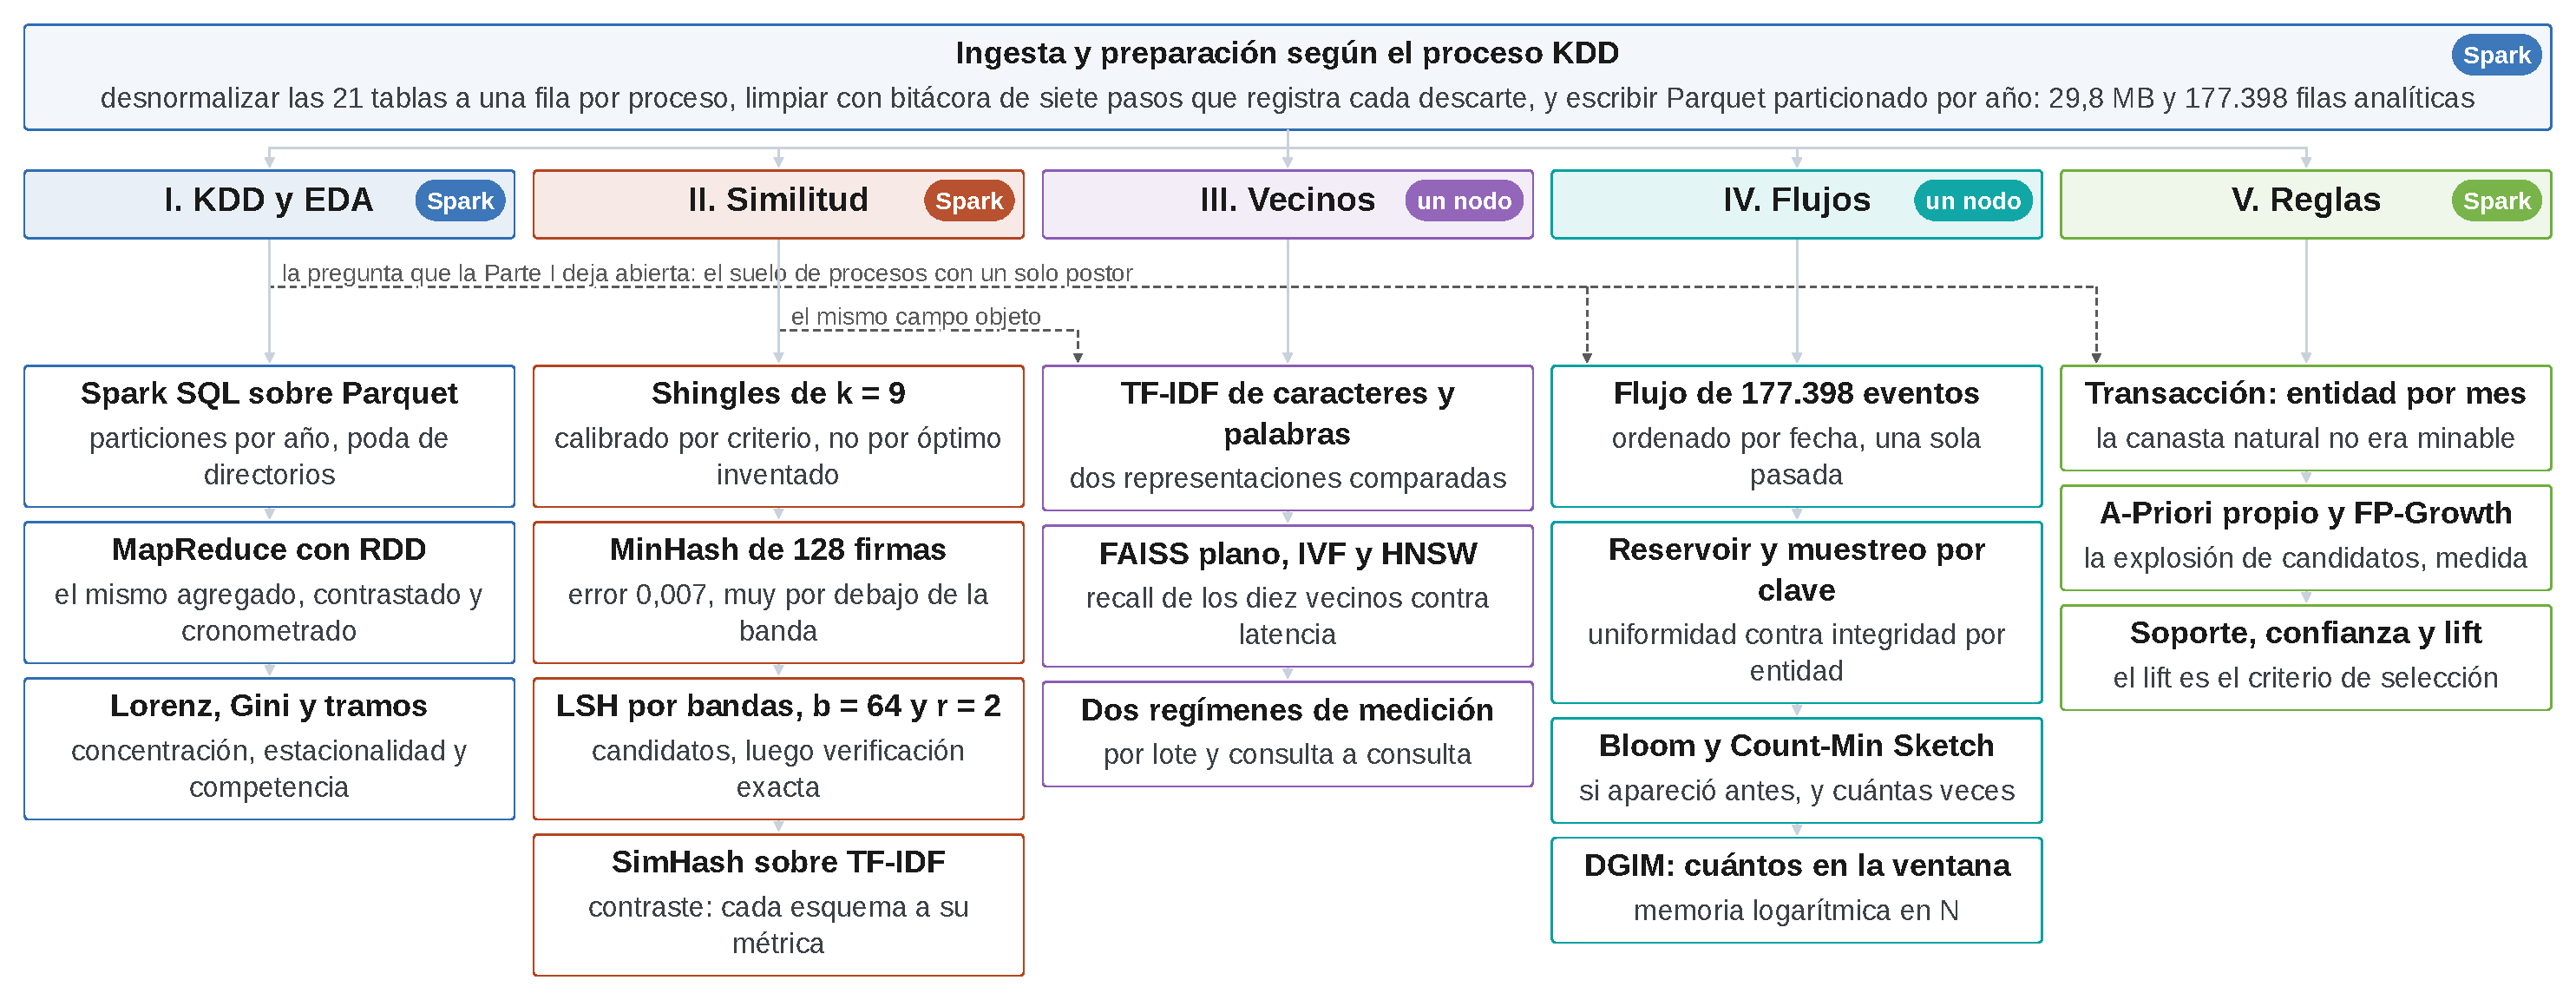
\includegraphics[height=0.74\textheight,width=\textwidth,keepaspectratio]{../figs/arquitectura_diapositiva.pdf}
  \end{center}
  \lectura{Lo único que viaja entre partes es la tabla analítica, de modo que son independientes; las líneas discontinuas marcan la pregunta que una parte deja abierta y otra recoge.}
\end{frame}

\begin{frame}{Cada decisión de limpieza queda registrada}
  \framesubtitle{Parte I \textperiodcentered{} KDD}
  \begin{center}
  \footnotesize
  \begin{tabular}{llrr}
    \toprule
    \textbf{Paso} & \textbf{Qué hace} & \textbf{Filas afectadas} & \textbf{Quedan} \\
    \midrule
    entrada & tabla analitica cruda & 0 & 281.462 \\
    duplicados & una fila por ocid, la mas reciente & 0 & 281.462 \\
    descarte & monto\_pen nulo o no positivo & 22.830 & 258.632 \\
    descarte & fecha fuera de 2023 a 2025 & 81.234 & 177.398 \\
    imputacion & n\_postores con la mediana de su metodo & 6.655 & 177.398 \\
    marca & monto fuera de [6.37, 17.99] en escala log,… & 565 & 177.398 \\
    recorte & n\_postores winsorizado al percentil 99,9, t… & 263 & 177.398 \\
    \bottomrule
  \end{tabular}
  \end{center}
  \lectura{El motor de limpieza devuelve una bitácora, de modo que ningún descarte queda escondido en el código.}
\end{frame}

\begin{frame}{Dos decisiones cuestan el 37 por ciento de las filas}
  \framesubtitle{Parte I \textperiodcentered{} KDD}
  \begin{center}
    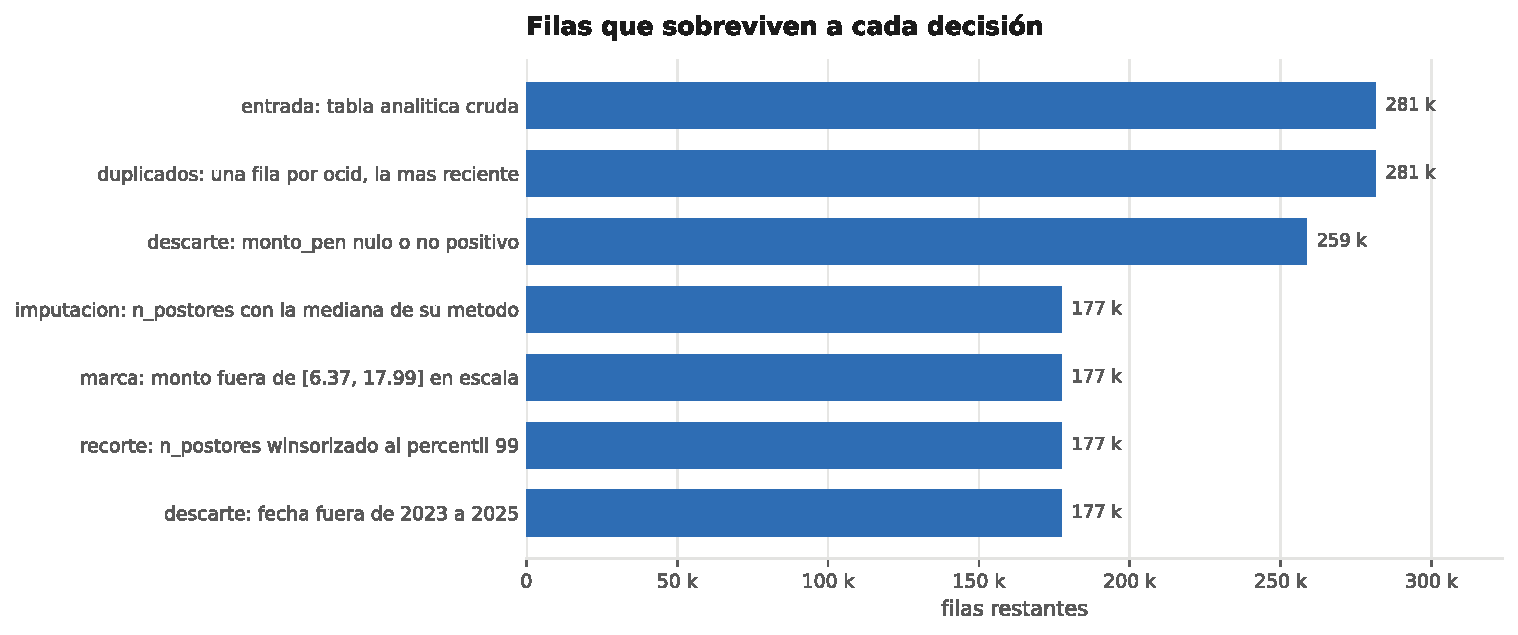
\includegraphics[height=0.74\textheight,width=\textwidth,keepaspectratio]{../figs/f02_embudo.pdf}
  \end{center}
  \lectura{Se descartan los montos no positivos, que son campos no publicados, y las convocatorias fuera de la ventana 2023 a 2025.}
\end{frame}

\begin{frame}{Diciembre es el máximo en los dos años completos}
  \framesubtitle{Parte I \textperiodcentered{} EDA}
  \begin{center}
    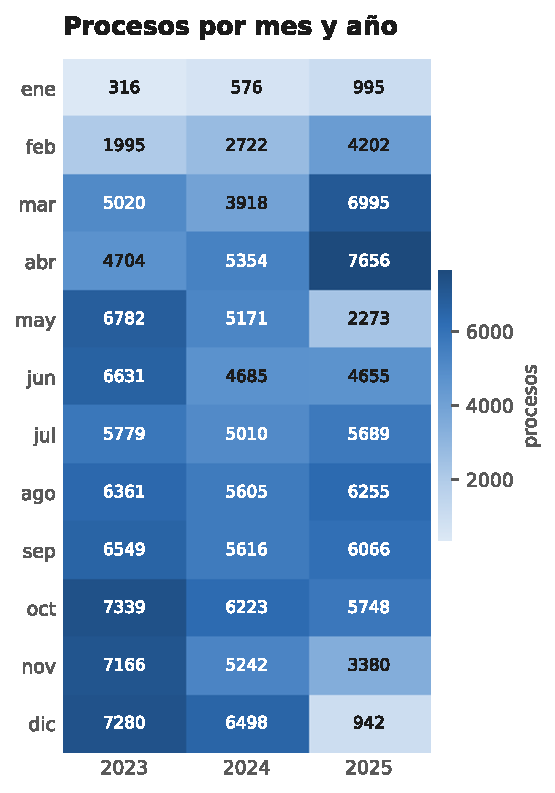
\includegraphics[height=0.74\textheight,width=\textwidth,keepaspectratio]{../figs/f05_estacionalidad.pdf}
  \end{center}
  \lectura{El patrón se repite en 2023 y 2024, lo que permite atribuirlo al cierre presupuestal y no al ruido de un año.}
\end{frame}

\begin{frame}{El uno por ciento de proveedores concentra el 47 por ciento del monto}
  \framesubtitle{Parte I \textperiodcentered{} EDA}
  \begin{center}
    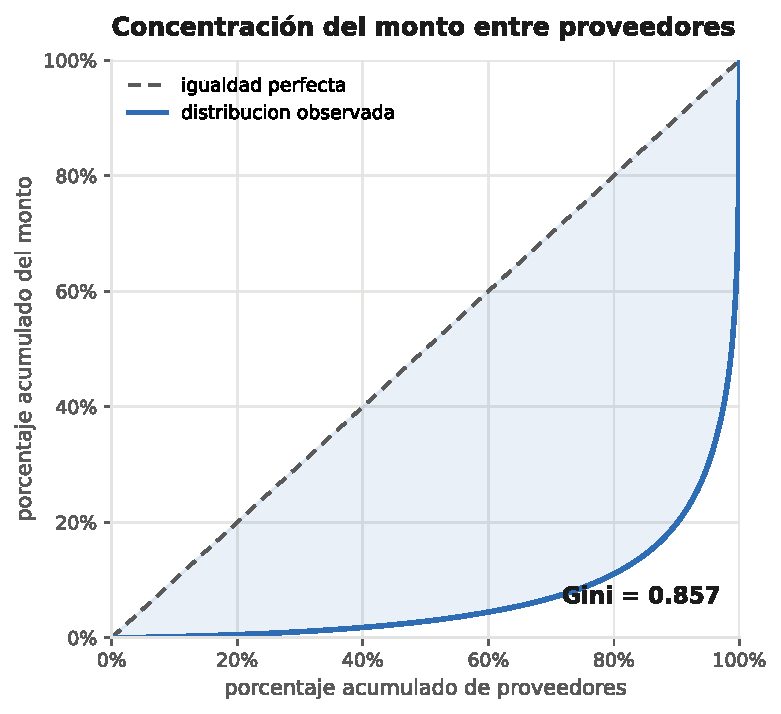
\includegraphics[height=0.74\textheight,width=\textwidth,keepaspectratio]{../figs/f11_lorenz.pdf}
  \end{center}
  \lectura{El coeficiente de Gini es 0,857 sobre un máximo de 1.}
\end{frame}

\begin{frame}{El Gini nacional no describe a un mercado regional típico}
  \framesubtitle{Parte I \textperiodcentered{} EDA}
  \begin{center}
    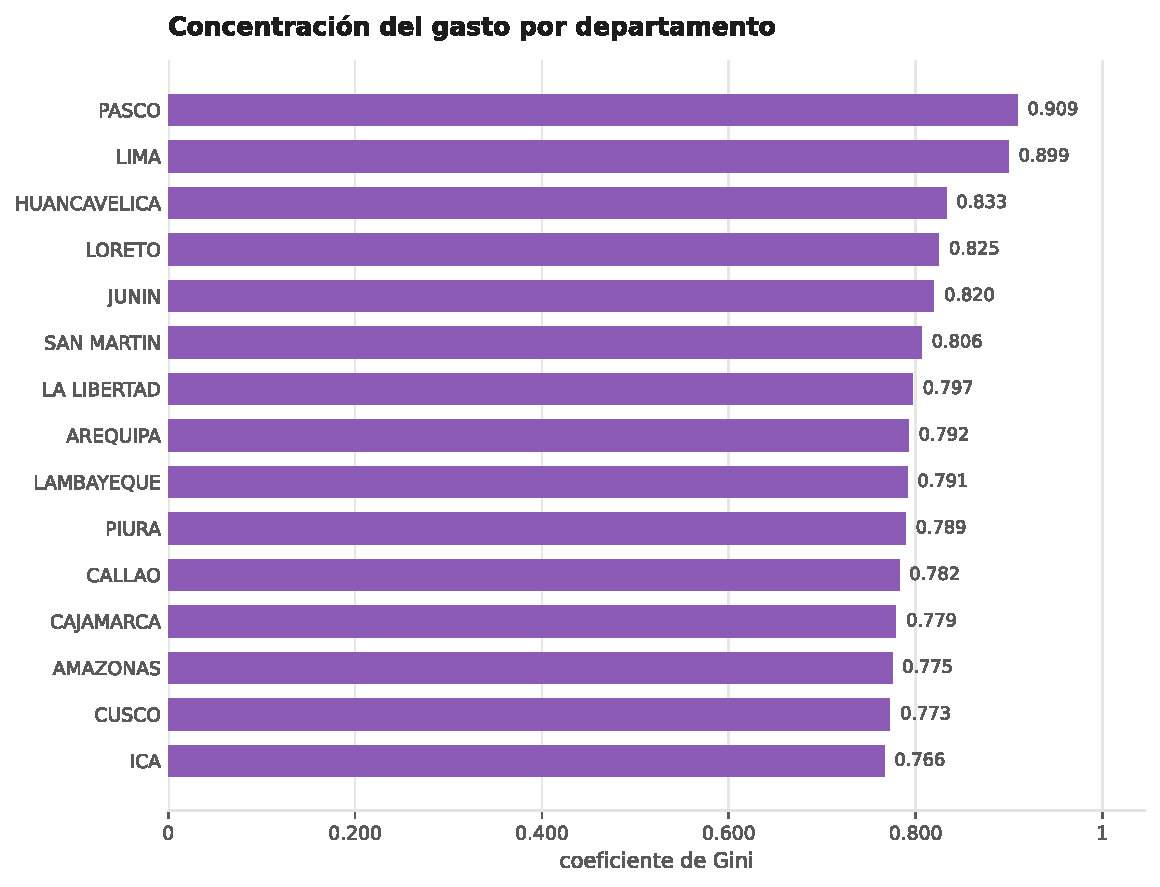
\includegraphics[height=0.74\textheight,width=\textwidth,keepaspectratio]{../figs/f12_gini_departamento.pdf}
  \end{center}
  \lectura{Solo Pasco y Lima superan el valor nacional, y el resto queda por debajo: la cifra del país está empujada por Lima.}
\end{frame}

\begin{frame}{La falta de competencia tiene dos formas distintas}
  \framesubtitle{Parte I \textperiodcentered{} EDA}
  \begin{center}
    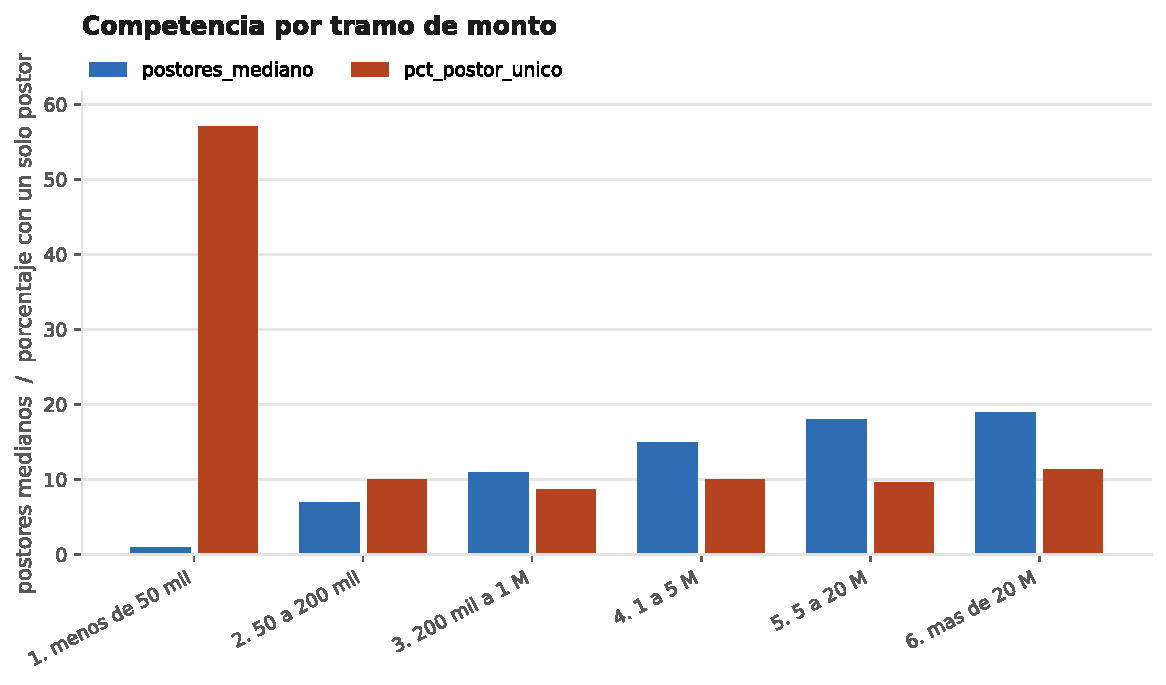
\includegraphics[height=0.74\textheight,width=\textwidth,keepaspectratio]{../figs/f13_competencia.pdf}
  \end{center}
  \lectura{Bajo cincuenta mil soles el 57 por ciento tuvo un solo postor, y en el resto de tramos se estabiliza cerca del 10 por ciento.}
\end{frame}

\begin{frame}{MapReduce sobre RDD frente a DataFrames}
  \framesubtitle{Parte I \textperiodcentered{} Spark}
  \begin{center}
    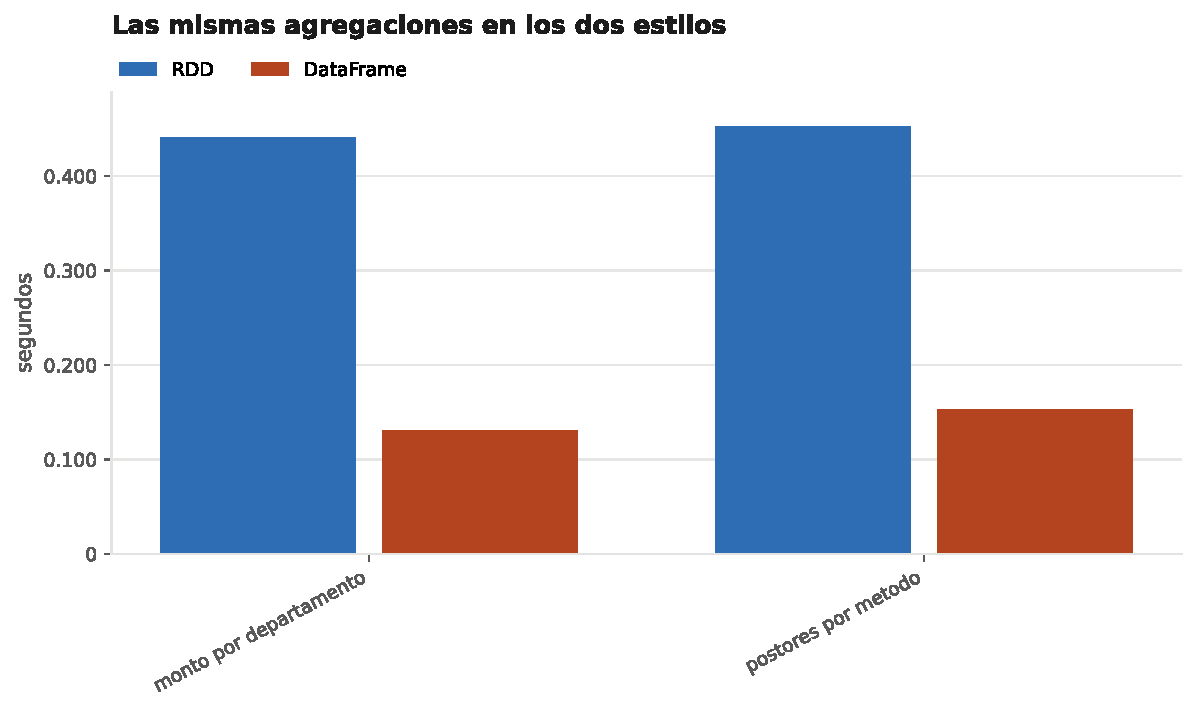
\includegraphics[height=0.74\textheight,width=\textwidth,keepaspectratio]{../figs/f14_rdd_vs_dataframe.pdf}
  \end{center}
  \lectura{El mismo resultado, verificado con exceptAll en ambos sentidos, cuesta tres veces más en RDD por la serialización hacia Python.}
\end{frame}

\begin{frame}{El particionado por año permite descartar directorios}
  \framesubtitle{Parte I \textperiodcentered{} Spark}
  \begin{center}
    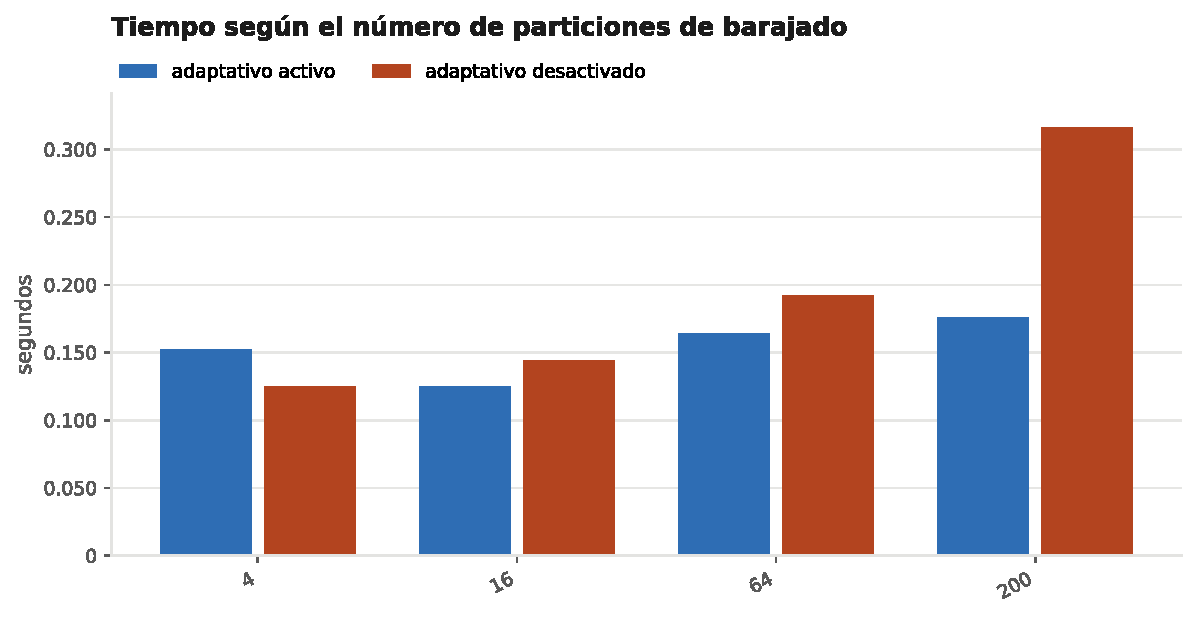
\includegraphics[height=0.74\textheight,width=\textwidth,keepaspectratio]{../figs/f15_shuffle.pdf}
  \end{center}
  \lectura{La ejecución adaptativa amortigua casi por completo una mala elección del número de particiones de barajado.}
\end{frame}

\begin{frame}{El tamaño del shingle no se optimiza, se fija con un criterio}
  \framesubtitle{Parte II \textperiodcentered{} Similitud}
  \begin{center}
    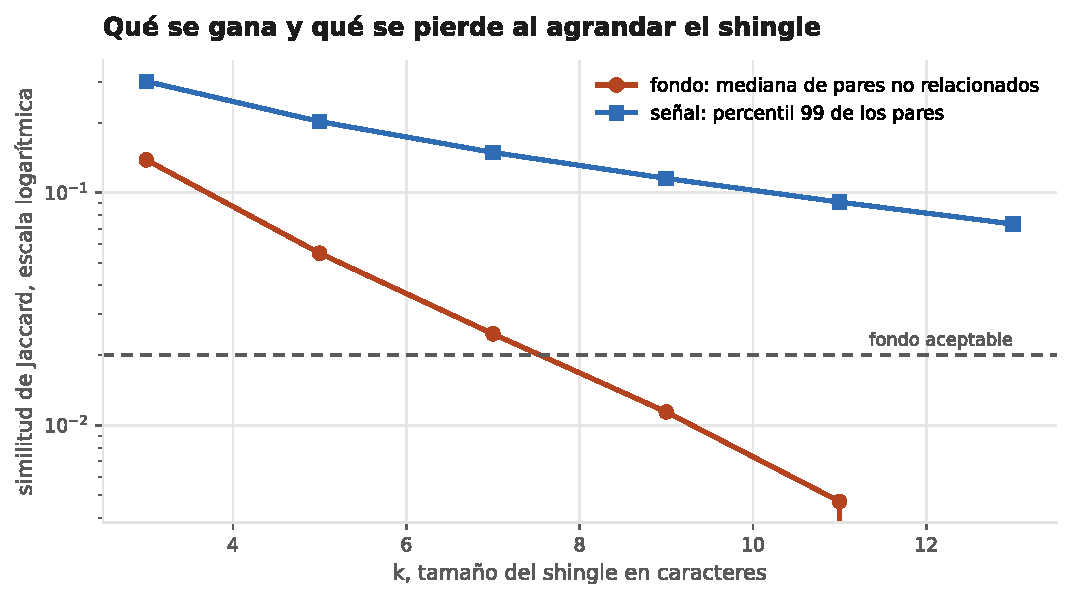
\includegraphics[height=0.74\textheight,width=\textwidth,keepaspectratio]{../figs/f16_calibracion_k.pdf}
  \end{center}
  \lectura{Las dos curvas bajan juntas, así que se toma el k más pequeño que deja el fondo de pares no relacionados por debajo de 0,02.}
\end{frame}

\begin{frame}{El error baja como uno sobre la raíz de n}
  \framesubtitle{Parte II \textperiodcentered{} MinHash}
  \begin{center}
    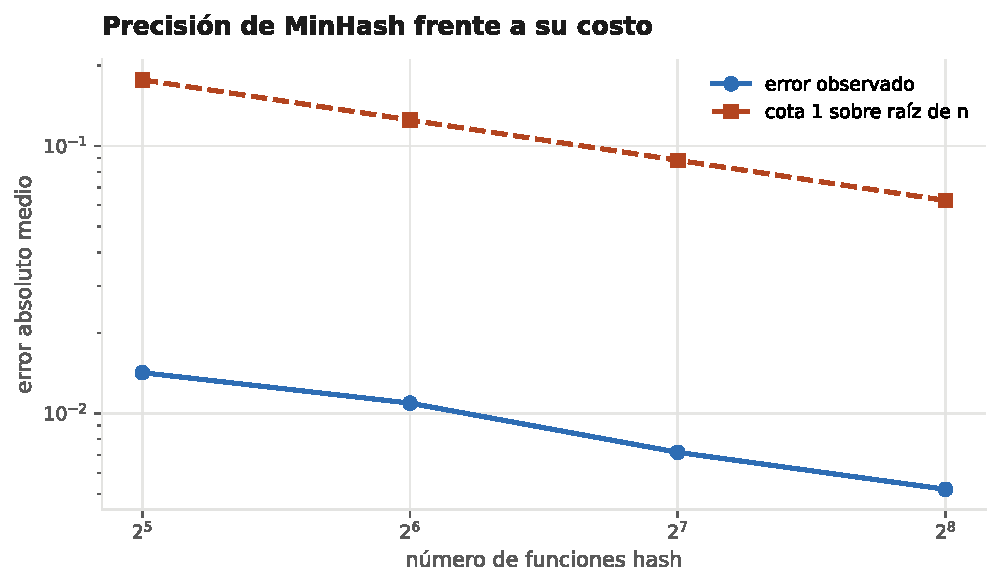
\includegraphics[height=0.74\textheight,width=\textwidth,keepaspectratio]{../figs/f18_error_minhash.pdf}
  \end{center}
  \lectura{Cuadruplicar las funciones hash solo divide el error entre dos, y con 128 ya queda por debajo del ancho de decisión de LSH.}
\end{frame}

\begin{frame}{Las bandas y las filas definen qué se considera parecido}
  \framesubtitle{Parte II \textperiodcentered{} LSH}
  \begin{center}
    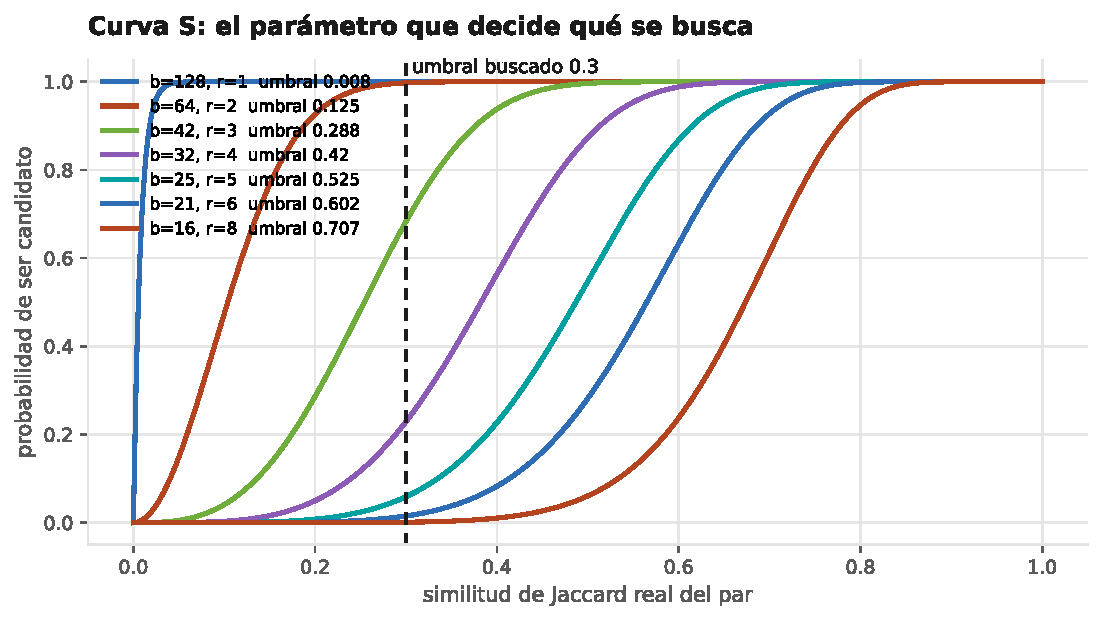
\includegraphics[height=0.74\textheight,width=\textwidth,keepaspectratio]{../figs/f19_curva_s.pdf}
  \end{center}
  \lectura{El umbral teórico marca el cambio de concavidad de la curva, donde la probabilidad vale 1 menos 1 sobre e y no un medio.}
\end{frame}

\begin{frame}{Falsos positivos frente a falsos negativos}
  \framesubtitle{Parte II \textperiodcentered{} LSH}
  \begin{center}
  \footnotesize
  \begin{tabular}{lrrrrr}
    \toprule
    \textbf{Configuración} & \textbf{Candidatos} & \textbf{Falsos pos.} & \textbf{Falsos neg.} & \textbf{Recall} & \textbf{\% a verificar} \\
    \midrule
    b=128, r=1 & 993.962 & 993.699 & 0 & 1,0000 & 49,7230 \\
    b=64, r=2 & 171.259 & 170.997 & 1 & 0,9962 & 8,5670 \\
    b=42, r=3 & 32.337 & 32.106 & 32 & 0,8783 & 1,6180 \\
    b=32, r=4 & 1.177 & 1.051 & 137 & 0,4791 & 0,0590 \\
    b=25, r=5 & 139 & 64 & 188 & 0,2852 & 0,0070 \\
    b=21, r=6 & 59 & 18 & 222 & 0,1559 & 0,0030 \\
    b=16, r=8 & 24 & 0 & 239 & 0,0913 & 0,0010 \\
    \bottomrule
  \end{tabular}
  \end{center}
  \lectura{Un falso positivo lo elimina la verificación exacta posterior y es solo trabajo; un falso negativo se pierde para siempre.}
\end{frame}

\begin{frame}{Un caso concreto encontrado por el método}
  \framesubtitle{Parte II \textperiodcentered{} LSH}
  \begin{center}
  \scriptsize
  \begin{tabular}{rll}
    \toprule
    \textbf{Jaccard} & \textbf{Entidad A} & \textbf{Entidad B} \\
    \midrule
    1,000 & AUTORIDAD NACIONAL DEL AGUA & AUTORIDAD NACIONAL DEL AGUA \\
    1,000 & CENTRO NACIONAL DE ABASTECIMIENTO D… & CENTRO NACIONAL DE ABASTECIMIENTO D… \\
    0,963 & MUNICIPALIDAD DISTRITAL DE TAMBO DE… & MUNICIPALIDAD DISTRITAL DE SAN BART… \\
    0,934 & UNIDAD EJECUTORA 003 GESTION INTEGR… & UNIDAD EJECUTORA 003 GESTION INTEGR… \\
    0,869 & COMISION DE PROMOCION DEL PERU PARA… & COMISION DE PROMOCION DEL PERU PARA… \\
    \bottomrule
  \end{tabular}
  \end{center}
  \lectura{Los pares de la misma entidad son reconvocatorias del mismo objeto, y el de Tambo de Mora con San Bartolo son dos municipalidades distintas que comparten el pliego del programa Vaso de Leche, lo que indica una plantilla reutilizada y no una irregularidad.}
\end{frame}

\begin{frame}{El régimen de medición cambia la conclusión}
  \framesubtitle{Parte III \textperiodcentered{} ANN}
  \begin{center}
    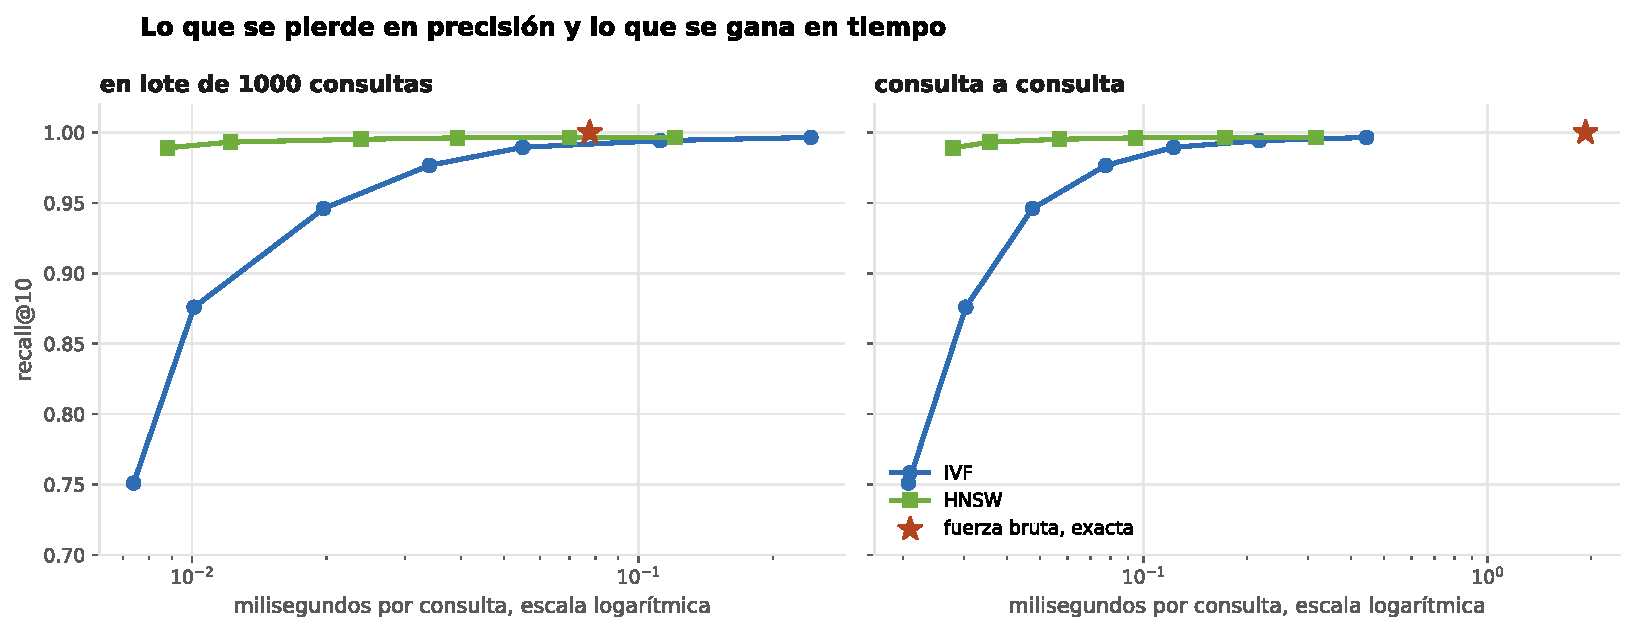
\includegraphics[height=0.74\textheight,width=\textwidth,keepaspectratio]{../figs/f24_ann_vs_exacta.pdf}
  \end{center}
  \lectura{En lote el índice aproximado no aporta nada, y consulta a consulta HNSW es un orden de magnitud más rápido.}
\end{frame}

\begin{frame}{Por qué existen los índices aproximados}
  \framesubtitle{Parte III \textperiodcentered{} ANN}
  \begin{center}
    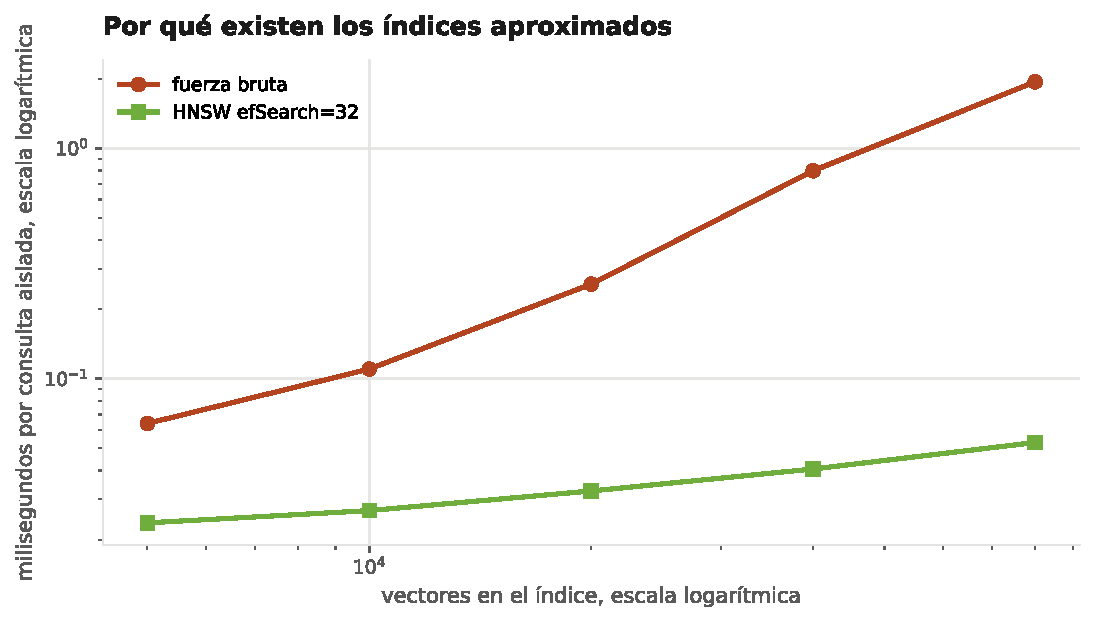
\includegraphics[height=0.74\textheight,width=\textwidth,keepaspectratio]{../figs/f26_escalado.pdf}
  \end{center}
  \lectura{La búsqueda exacta crece de forma lineal con la base y HNSW casi no crece, así que la ventaja aparece al escalar.}
\end{frame}

\begin{frame}{El filtro de Bloom respeta su tasa teórica}
  \framesubtitle{Parte IV \textperiodcentered{} Flujos}
  \begin{center}
    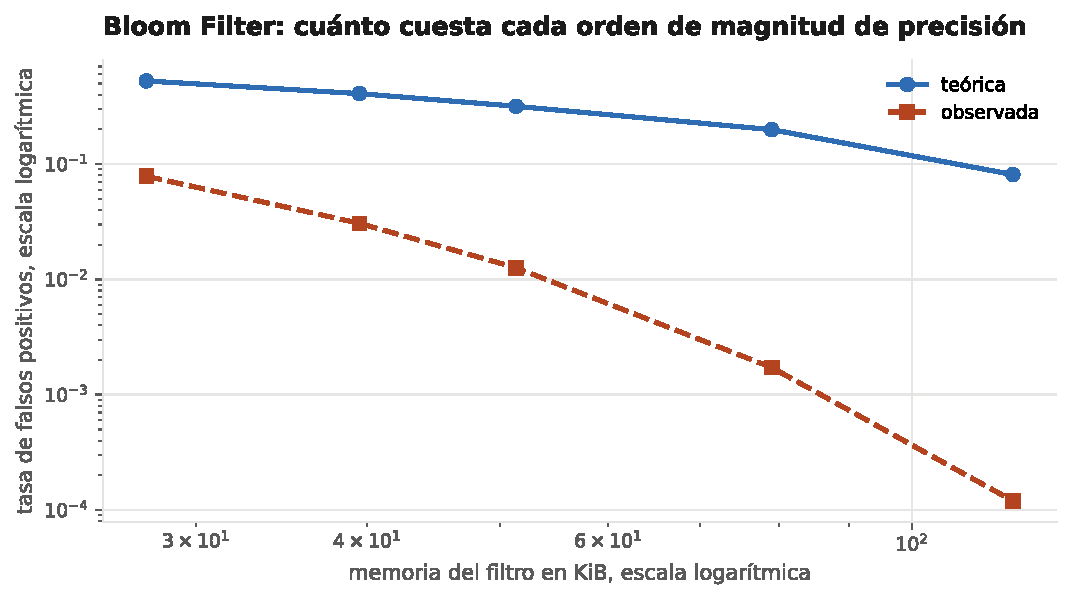
\includegraphics[height=0.74\textheight,width=\textwidth,keepaspectratio]{../figs/f29_bloom.pdf}
  \end{center}
  \lectura{Cada orden de magnitud de precisión cuesta unos diez bits más por elemento, y los falsos negativos son imposibles.}
\end{frame}

\begin{frame}{Por qué hacen falta Bloom y Count-Min, no uno de los dos}
  \framesubtitle{Parte IV \textperiodcentered{} Flujos}
  \begin{center}
    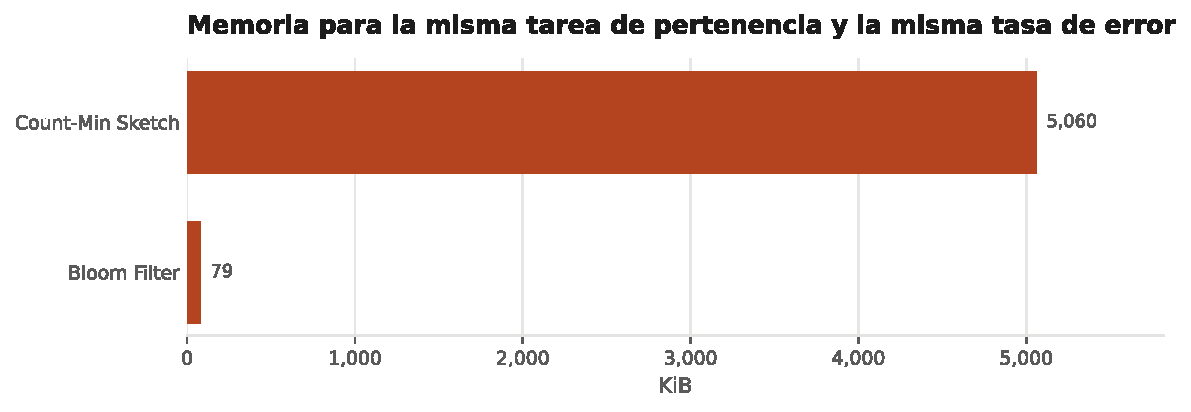
\includegraphics[height=0.74\textheight,width=\textwidth,keepaspectratio]{../figs/f31_bloom_vs_cms.pdf}
  \end{center}
  \lectura{Con la misma tasa de error, el Count-Min necesita sesenta y cuatro veces más memoria para responder pertenencia.}
\end{frame}

\begin{frame}{DGIM sobre la ventana reciente}
  \framesubtitle{Parte IV \textperiodcentered{} Flujos}
  \begin{center}
    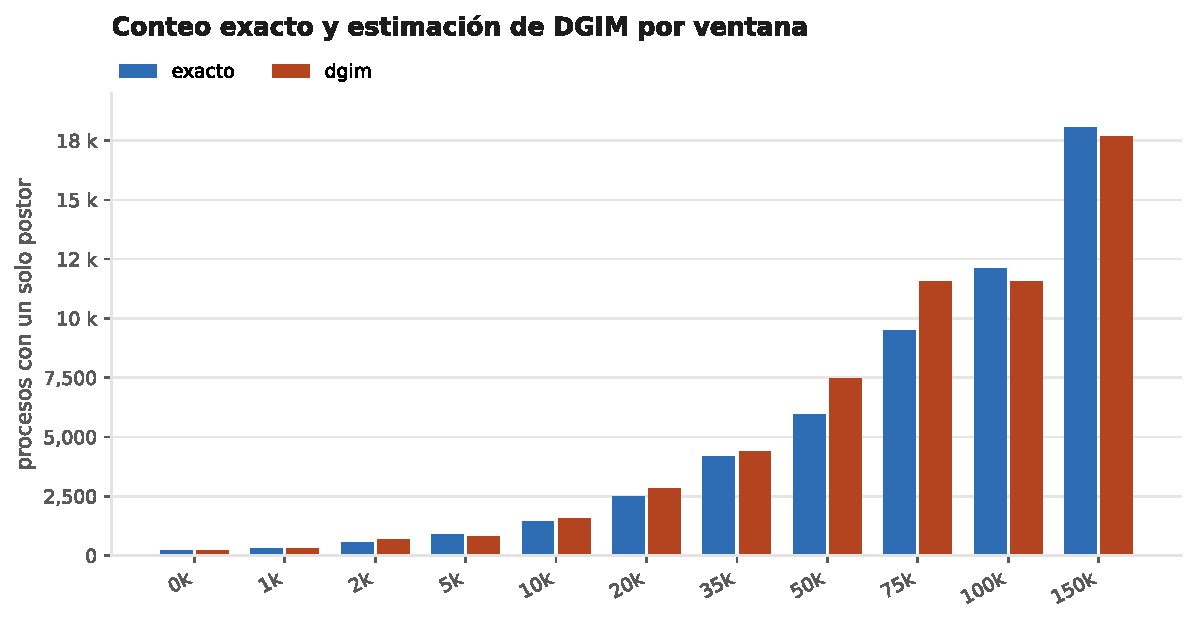
\includegraphics[height=0.74\textheight,width=\textwidth,keepaspectratio]{../figs/f32_dgim.pdf}
  \end{center}
  \lectura{El peor error observado queda muy por debajo de la cota del cincuenta por ciento que garantizan dos cubos por tamaño.}
\end{frame}

\begin{frame}{El tiempo es la tercera dimensión del compromiso}
  \framesubtitle{Parte IV \textperiodcentered{} Flujos}
  \begin{center}
    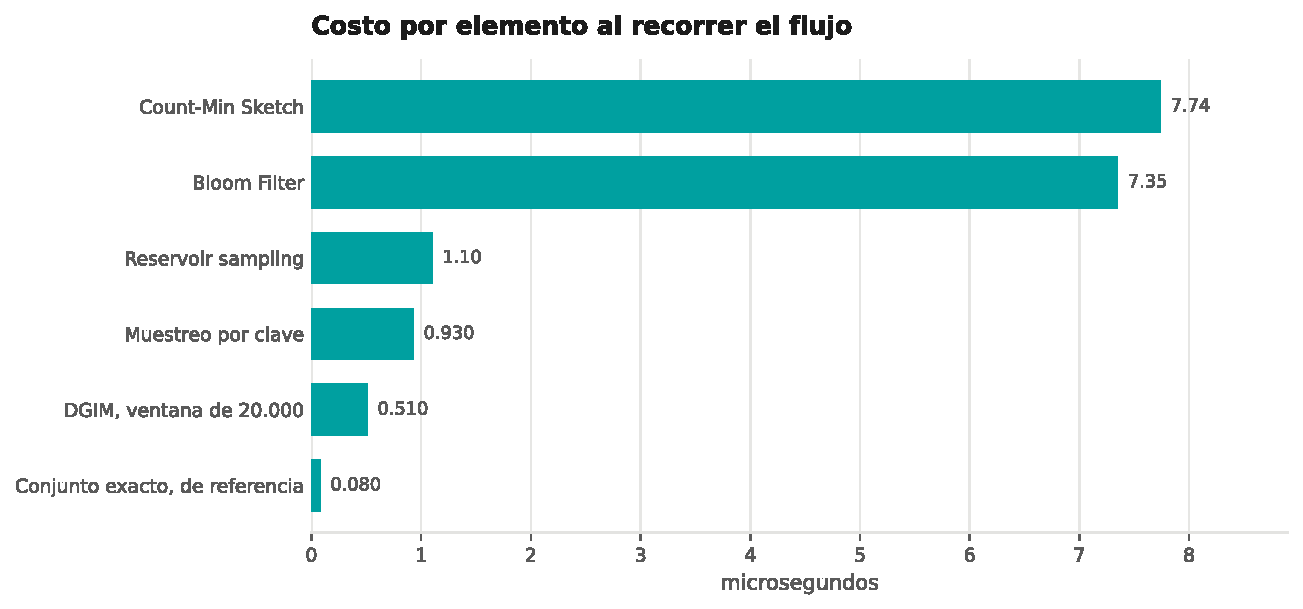
\includegraphics[height=0.74\textheight,width=\textwidth,keepaspectratio]{../figs/f38_tiempos_estructuras.pdf}
  \end{center}
  \lectura{Estas estructuras no ahorran tiempo: cambian memoria por tiempo y por un error acotado.}
\end{frame}

\begin{frame}{Las cinco estructuras, lado a lado}
  \framesubtitle{Parte IV \textperiodcentered{} Flujos}
  \begin{center}
  \scriptsize
  \begin{tabular}{llll}
    \toprule
    \textbf{Estructura} & \textbf{Qué pregunta responde} & \textbf{Memoria} & \textbf{Tiempo} \\
    \midrule
    Muestreo por clave & métricas por entidad sobre una muestra & proporcional a la fracción de claves & 0.93 us \\
    Reservoir sampling & proporciones sobre todo el flujo & k elementos, fija y conocida de antemano & 1.10 us \\
    Bloom Filter & apareció antes este proveedor & 79.0 KiB para 67,510 claves & 7.35 us \\
    Count-Min Sketch & cuántas veces apareció cada ítem & 149 KiB & 7.74 us \\
    DGIM & cuántos en los últimos N elementos & 20 cubos para N=150,000 & 0.51 us \\
    \bottomrule
  \end{tabular}
  \end{center}
  \lectura{Ninguna sustituye a otra: responden preguntas distintas sobre el mismo flujo.}
\end{frame}

\begin{frame}{La definición de transacción era el problema}
  \framesubtitle{Parte V \textperiodcentered{} Reglas}
  \begin{center}
    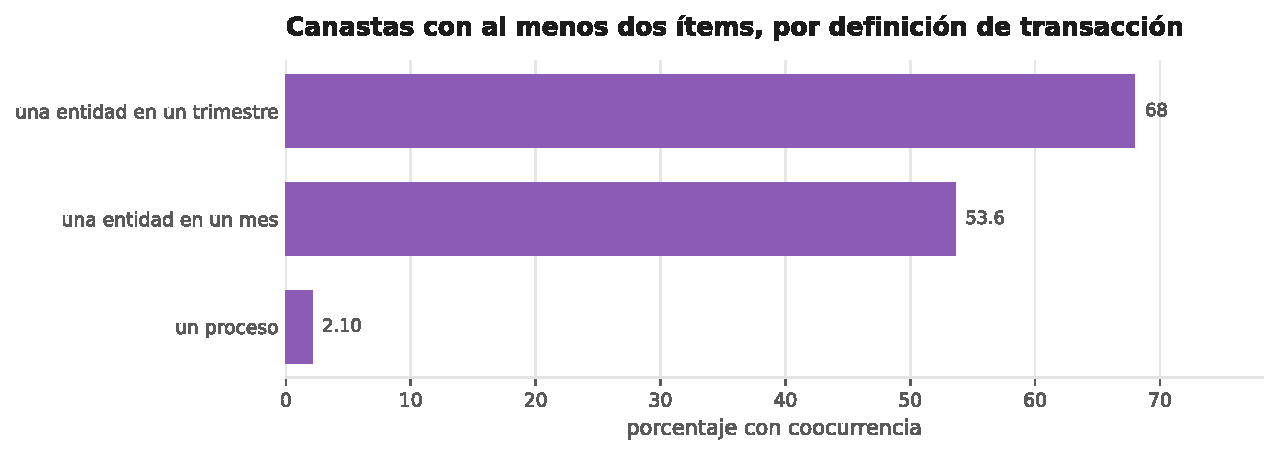
\includegraphics[height=0.74\textheight,width=\textwidth,keepaspectratio]{../figs/f34_definicion_transaccion.pdf}
  \end{center}
  \lectura{La canasta natural tiene coocurrencia en el 2 por ciento de los procesos, así que se redefine como lo que una entidad compra en un mes.}
\end{frame}

\begin{frame}{Por qué FP-Growth desplazó a A-Priori}
  \framesubtitle{Parte V \textperiodcentered{} Reglas}
  \begin{center}
    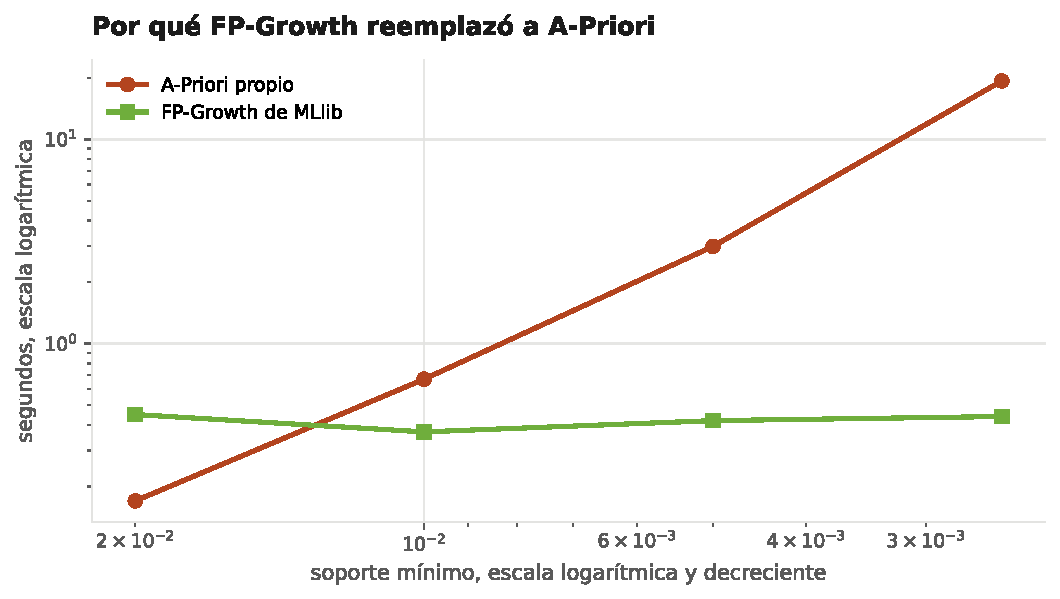
\includegraphics[height=0.74\textheight,width=\textwidth,keepaspectratio]{../figs/f35_apriori_vs_fpgrowth.pdf}
  \end{center}
  \lectura{Al bajar el umbral de soporte, A-Priori explota en candidatos y FP-Growth se mantiene plano.}
\end{frame}

\begin{frame}{Reglas con soporte, confianza y lift}
  \framesubtitle{Parte V \textperiodcentered{} Reglas}
  \begin{center}
  \footnotesize
  \begin{tabular}{llrrr}
    \toprule
    \textbf{Si compra} & \textbf{También compra} & \textbf{Soporte} & \textbf{Confianza} & \textbf{Lift} \\
    \midrule
    CONSERVA DE ENTERO DE SAR… & ACEITE VEGETAL COMESTIBLE & 0,0042 & 0,386 & 50,90 \\
    ACEITE VEGETAL COMESTIBLE & CONSERVA DE ENTERO DE SAR… & 0,0042 & 0,550 & 50,90 \\
    ACEITE VEGETAL COMESTIBLE & ARROZ PILADO SUPERIOR & 0,0047 & 0,616 & 37,85 \\
    ARROZ PILADO SUPERIOR & CONSERVA DE ENTERO DE SAR… & 0,0054 & 0,330 & 30,58 \\
    CONSERVA DE ENTERO DE SAR… & ARROZ PILADO SUPERIOR & 0,0054 & 0,498 & 30,58 \\
    SERVICIO DE ALQUILER DE C… & SERVICIO DE ALQUILER DE E… & 0,0043 & 0,705 & 18,13 \\
    SERVICIO DE ALQUILER DE C… & SERVICIO DE ALQUILER DE E… & 0,0089 & 0,604 & 15,54 \\
    HOJUELA DE AVENA, QUINUA… & LECHE EVAPORADA ENTERA X… & 0,0160 & 0,697 & 8,81 \\
    \bottomrule
  \end{tabular}
  \end{center}
  \lectura{El lift es el criterio de selección: una confianza alta sobre un ítem ya frecuente no dice nada.}
\end{frame}

\begin{frame}{Dónde se concentra la falta de competencia}
  \framesubtitle{Parte V \textperiodcentered{} Reglas}
  \begin{center}
    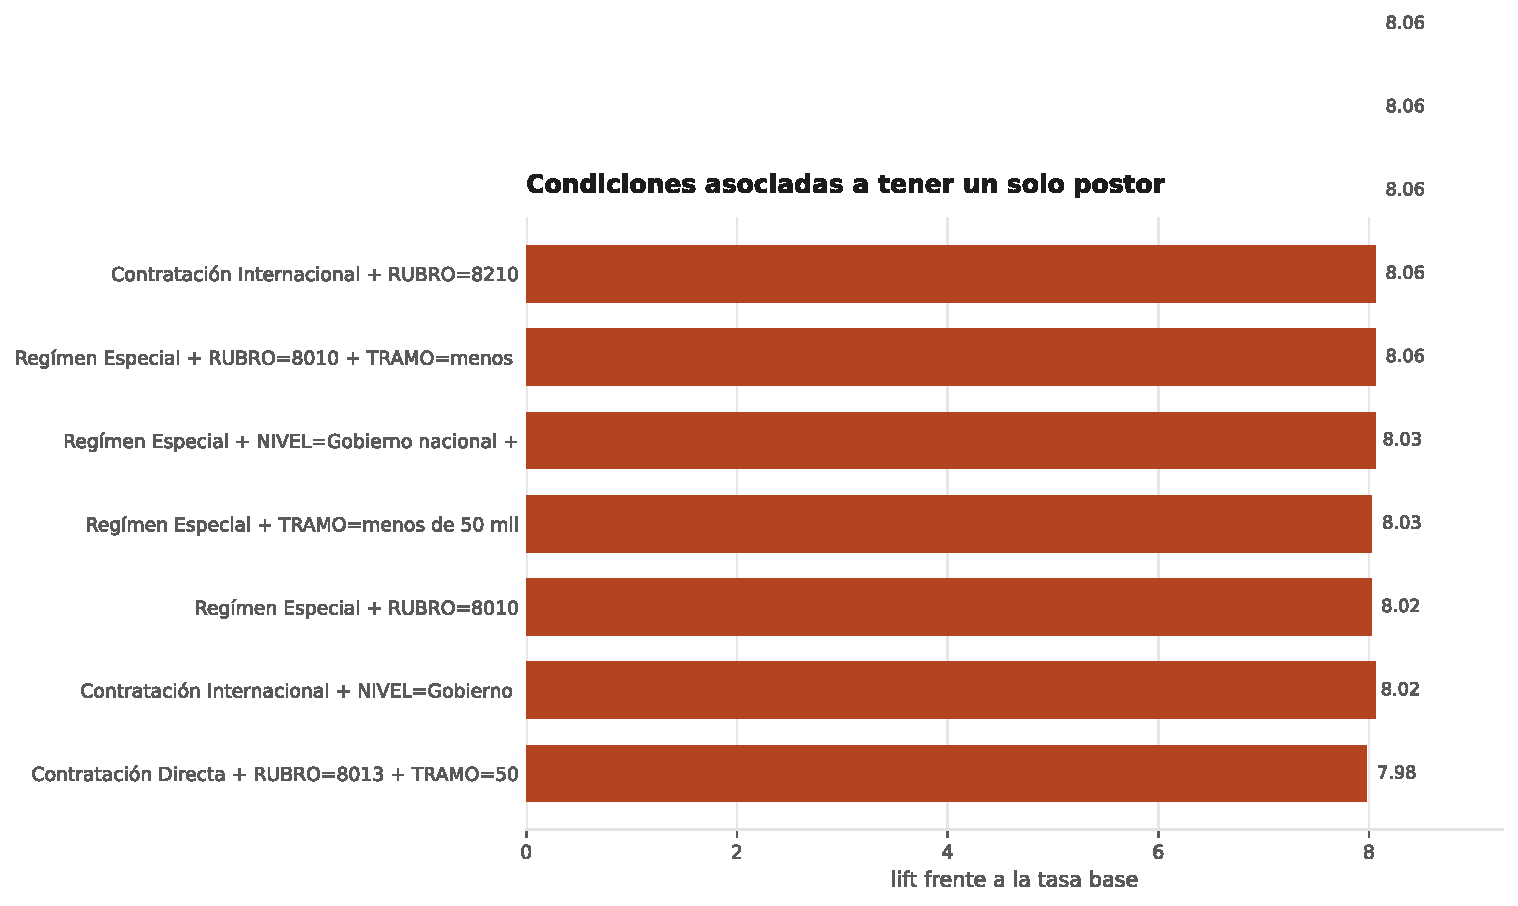
\includegraphics[height=0.74\textheight,width=\textwidth,keepaspectratio]{../figs/f37_postor_unico.pdf}
  \end{center}
  \lectura{El suelo de procesos sin competencia no se reparte al azar, aunque parte de lo que aparece es administrativamente esperable.}
\end{frame}

\begin{frame}{Qué aportó cada técnica}
  \framesubtitle{Parte VI \textperiodcentered{} Discusión}
  \begin{itemize}\setlength{\itemsep}{0.7em}
    \item El EDA y la curva de Lorenz contestan la concentración con un número
    \item LSH aporta los candidatos de objetos duplicados
    \item Las reglas contestan dónde se concentra la falta de competencia
    \item La búsqueda de vecinos aportó poco a las preguntas y mucho al aprendizaje
  \end{itemize}
\end{frame}

\begin{frame}{Qué se benefició de Spark y qué no}
  \framesubtitle{Parte VI \textperiodcentered{} Discusión}
  \begin{itemize}\setlength{\itemsep}{0.7em}
    \item Sí: la ingesta, el EDA y el agrupamiento por bandas de LSH
    \item No: la búsqueda de vecinos, donde un nodo con FAISS es mejor herramienta
    \item No: la minería de flujos, cuyo recorrido es secuencial y con estado
    \item Afirmar que todo mejoró con Spark sería falso
  \end{itemize}
\end{frame}

\begin{frame}{Lo que este trabajo no autoriza a concluir}
  \framesubtitle{Parte VI \textperiodcentered{} Discusión}
  \begin{itemize}\setlength{\itemsep}{0.7em}
    \item Que dos objetos casi idénticos impliquen fraccionamiento o colusión
    \item Que una concentración alta implique conducta anticompetitiva
    \item Que una regla con lift alto implique causalidad
    \item Que estas cifras sean oficiales: describen el paquete descargado
  \end{itemize}
\end{frame}

\begin{frame}{Entregables}
  \framesubtitle{Cierre}
  \begin{itemize}\setlength{\itemsep}{0.7em}
    \item Seis notebooks ejecutados, uno por parte, con sus módulos de apoyo
    \item Documento con la justificación detallada de cada decisión
    \item Informe de seis páginas con la propuesta y los hallazgos
    \item Reporte web interactivo con quince figuras y seis parámetros ajustables en vivo
  \end{itemize}
\end{frame}

\end{document}